\chapter{Supplemental Information}

\raggedbottom


%%%%%%%%%%%%%%%%%%%%%%%%%%%

%%%%%%%%%%%%%%%%%%%%%%%%%%%_________________CHAPTERTWO_________________%%%%%%%%%%%%%%%%%%%%%%%%%%%

%%%%%%%%%%%%%%%%%%%%%%%%%%%
\clearpage
\section{Appendix for Chapter 2}
\subsection{Supplemental Figures}
%Supplemental Figure 1: Histogram of TPM distribution
\begin{figure}[h!]
  \centering
    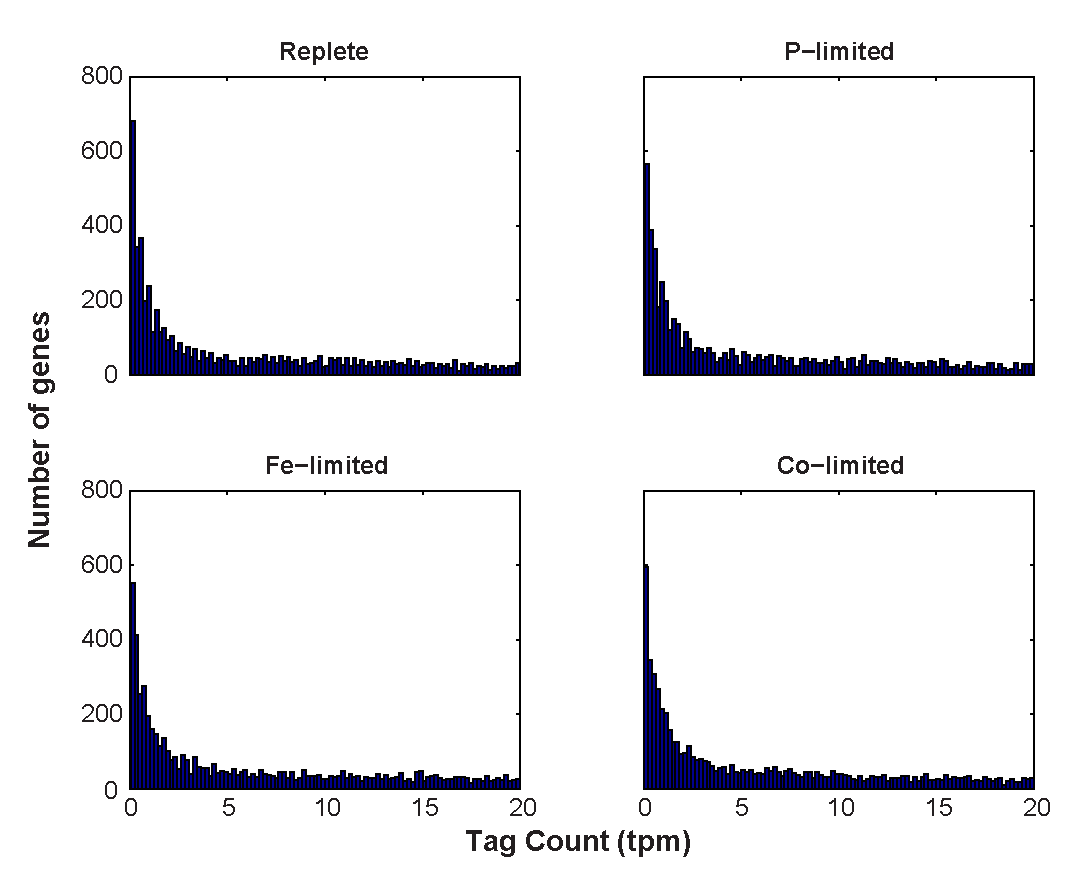
\includegraphics[width=1\textwidth]{Images/C2_FigureS1_v6.pdf}
    \caption[Distribution of normalized tag counts across treatments]{Histogram analysis of the distribution of normalized tag counts (TPM) for each gene across each of the four treatments (Replete, P-limited, Fe-limited, and co-limited). The abundance of normalized tag counts (TPM) was assessed, tallying the total number of genes with a given tag count. Only tag counts less than 20 are depicted to aid the visualization of the inflection in the data at 2.5 TPM.}
  \label{fig:a1f1}
\end{figure}

%Supplemental Figure 2: K-means clusters (all)
\begin{landscape}
   \null         %%<---- this is needed
   \vfill        %%<-----here
   \centering 
    \begin{figure}
    \centering
        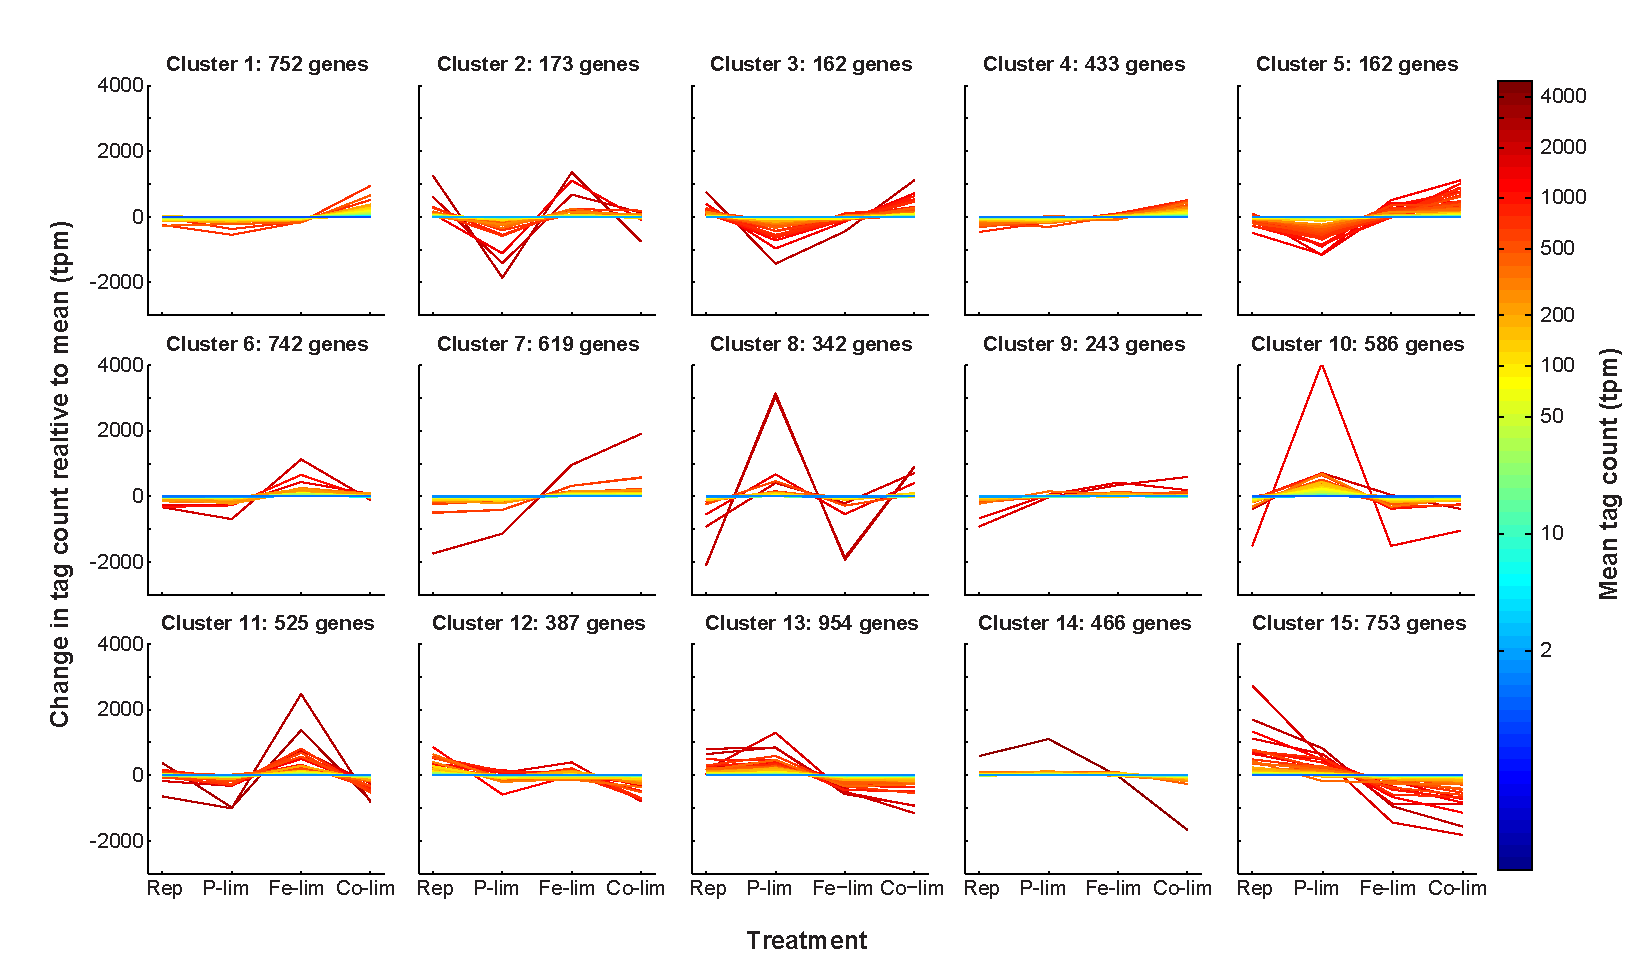
\includegraphics[width=1\textwidth]{Images/C2_FigureS2_v6.pdf}
        \caption[$K$-means clustering of normalized genes]{$K$-means clustering of normalized genes. The 7380 genes that passed the 2.5 TPM cutoff were clustered into 15 clusters using the $k$-means algorithm under the Pearson correlation coefficient. Tag counts normalized to total library size (in TPM) for each gene are plotted relative to the mean (indicated by the color of the line) for each of the four treatments: Replete (Rep), P-limited (P-lim), Fe-limited (Fe-lim), and co-limited (Co-lim).}
    \label{fig:a1f2} 
    \end{figure}
    \vfill        %%<----- and here
\end{landscape}

\clearpage
\subsection{Supplemental Data}

\newlist{DS2}{enumerate}{1}
\setlist[DS2]{label=Data Sheet 2-\arabic*}

    \begin{DS2}
    
    \item \label{DS21}: Genes in the \textit{T. pseudonana} genome homologous to reference genes from relative expression studies in algae and plants. \href{http://journal.frontiersin.org/file/downloadfile/16019/octet-stream/Data\%20Sheet\%201.XLS/313/2/31186}{Data Sheet 2-1} can be downloaded from the online version of the manuscript of \citet{Alexander2012} through \href{http://dx.doi.org/10.3389/fmicb.2012.00385}{Frontiers in Aquatic Microbiology}. 
    \item \label{DS22}: Putative reference genes identified with k-means clustering analysis (Cluster 9 and Clusters 14). \href{http://journal.frontiersin.org/file/downloadfile/16022/octet-stream/Data\%20Sheet\%202.XLS/313/1/31186}{Data Sheet 2-2} can be downloaded from the online version of the manuscript of \citet{Alexander2012} through \href{http://dx.doi.org/10.3389/fmicb.2012.00385}{Frontiers in Aquatic Microbiology}. 
        \item \label{DS23}: Data Sheet 3. Putative reference genes identified with ASC analysis ($p < 0.1$ for a fold change of 1.25). \href{http://journal.frontiersin.org/file/downloadfile/16025/octet-stream/Data\%20Sheet\%203.XLS/313/1/31186}{Data Sheet 2-3} can be downloaded from the online version of the manuscript of \citet{Alexander2012} through \href{http://dx.doi.org/10.3389/fmicb.2012.00385}{Frontiers in Aquatic Microbiology}. 

            \item \label{DS24}: The intersection of differentially expressed genes identified by \citet{Mock2008} and stably expressed genes identified through ASC (1.25 fold change bin, $p < 0.1$). \href{http://journal.frontiersin.org/file/downloadfile/16028/octet-stream/Data\%20Sheet\%204.XLS/313/1/31186}{Data Sheet 2-4} can be downloaded from the online version of the manuscript of \citet{Alexander2012} through \href{http://dx.doi.org/10.3389/fmicb.2012.00385}{Frontiers in Aquatic Microbiology}. 

    \end{DS2}


\newpage

%%%%%%%%%%%%%%%%%%%%%%%%%%%

%%%%%%%%%%%%%%%%%%%%%%%%%%%_________________CHAPTERTHREE_________________%%%%%%%%%%%%%%%%%%%%%%%%%%%

%%%%%%%%%%%%%%%%%%%%%%%%%%%


\section{Appendix for Chapter 3}
\subsection{Supplemental Figures}

%Supplemental Figure 1: Cell counts in NB 
\begin{figure}[h!]
  \centering
    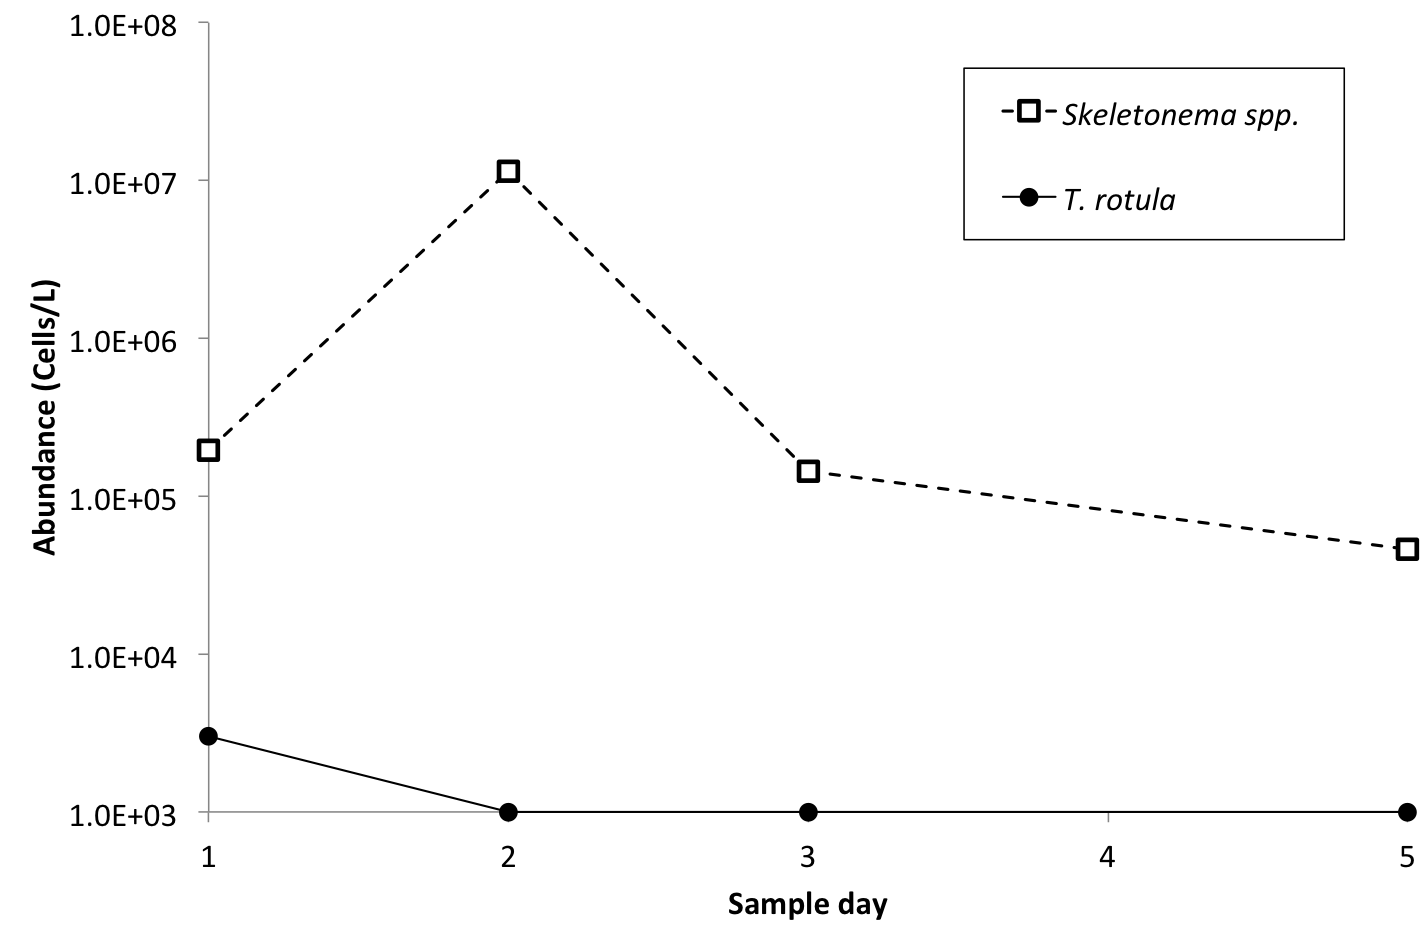
\includegraphics[width=1\textwidth]{Images/C3_SFigure1_CellCounts.png}
    \caption[Cell counts in Narragansett Bay during the spring of 2012]{Abundance estimation from cell counts of \textit{Skeletonema} spp. and \textit{T. rotula} across the five sample points during the spring of 2012. }
  \label{fig:a3f1}
\end{figure}


%Supplemental Figure 2: KEGG linear correlation
\begin{figure}[p!]
  \centering
    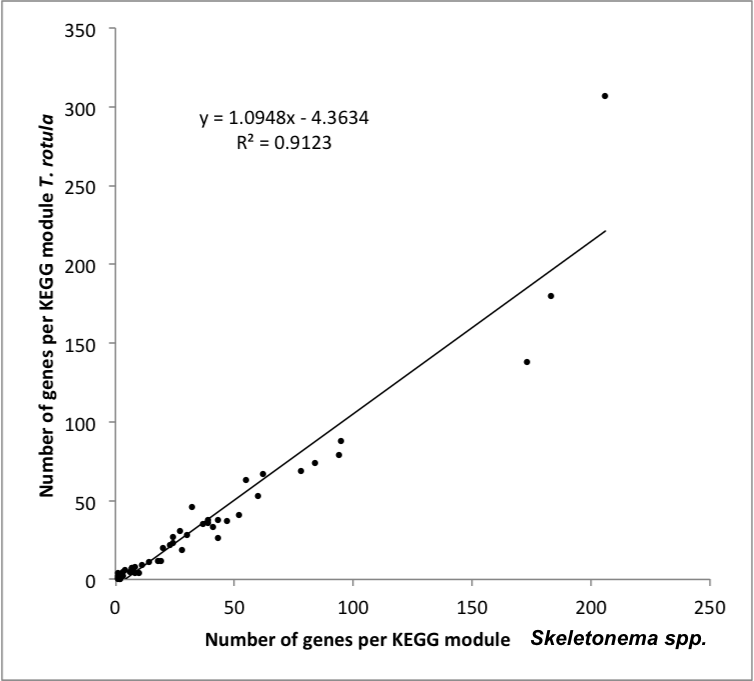
\includegraphics[width=1\textwidth]{Images/C3_SFigure2_KEGGModuleGeneContent2.png}
    \caption[Comparison of KEGG module content between \textit{Skeletonema} spp. and \textit{T. rotula} ]{Total number of genes assigned to each KEGG module for \textit{Skeletonema} spp. and \textit{T. rotula}.}
  \label{fig:a3f2}
\end{figure}


%Supplemental Figure 3: Hierarchical clustering of S and T across time
\begin{figure}[p!]
  \centering
    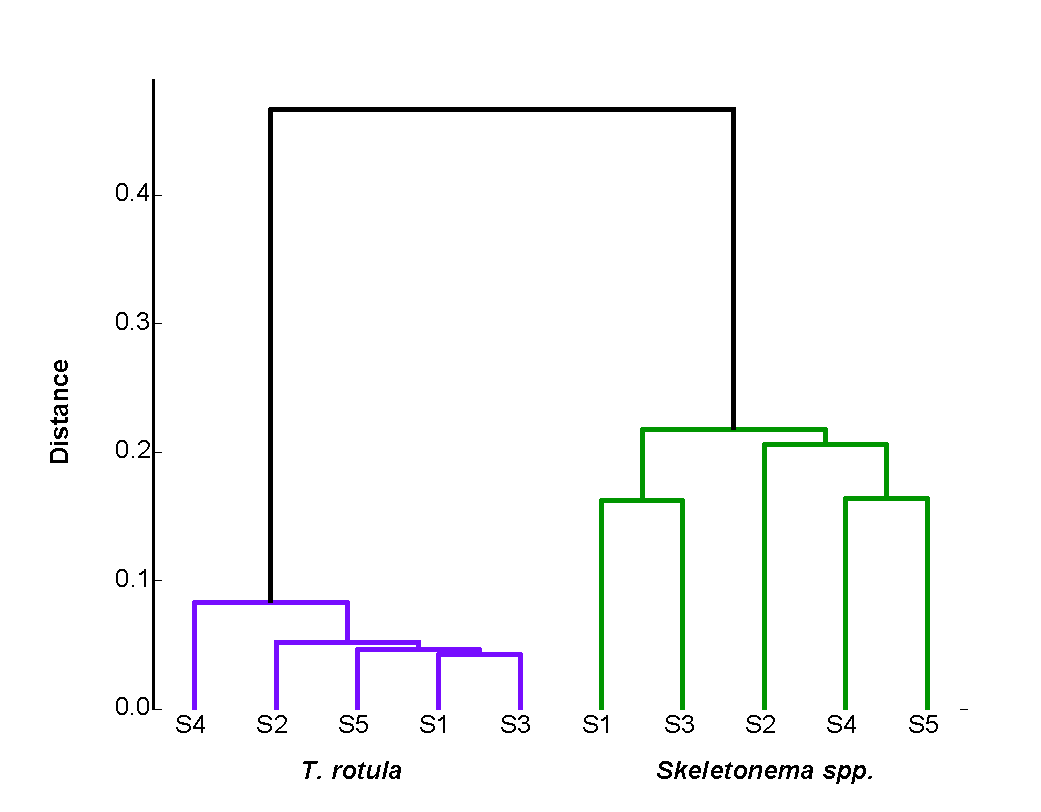
\includegraphics[width=1\textwidth]{Images/C3_SFigure3_Dendrogram.pdf}
    \caption[Hierarchical clustering of QMF signatures across species and samples]{Dendrogram depicting hierarchical clustering of samples based on relative expression of KEGG modules (Figure 2) across the five samples S1-S5 for \textit{Skeletonema} spp. and \textit{T. rotula}.}
  \label{fig:a3f3}
\end{figure}

%Supplemental Figure 4: Stable gene expression across time
\begin{figure}[p!]
  \centering
    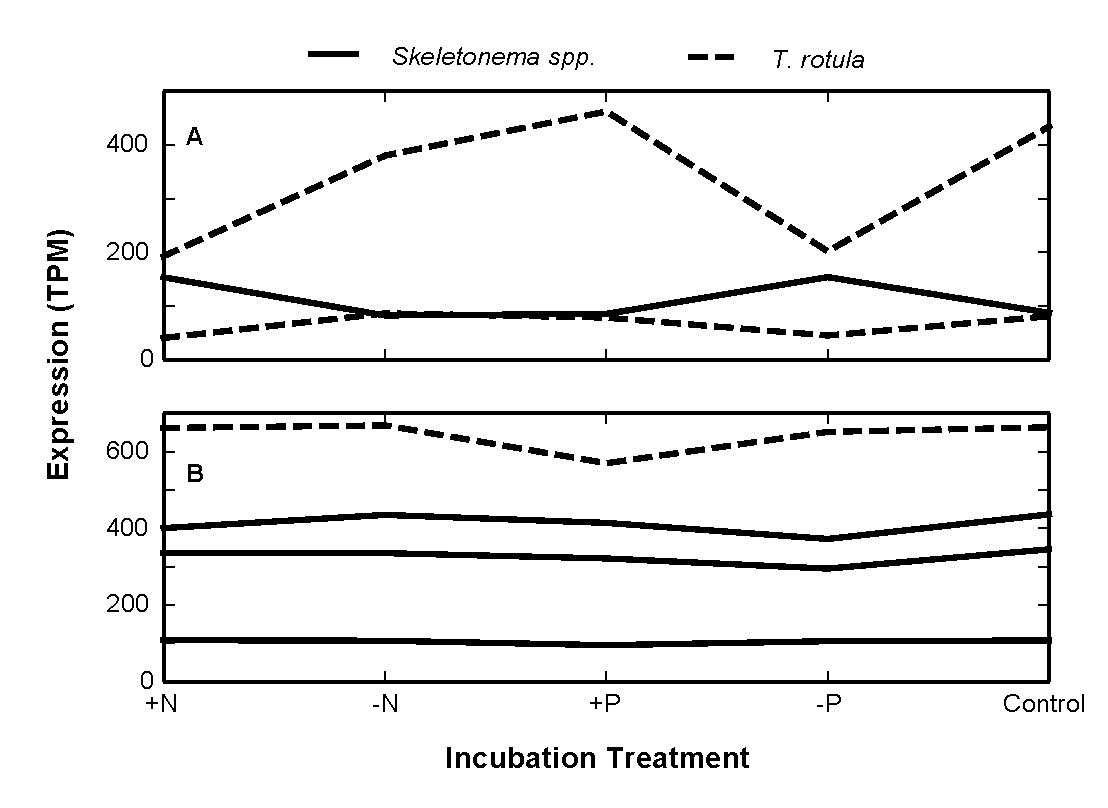
\includegraphics[width=1\textwidth]{Images/C3_SFigure4_StableGenePlot_wActin.pdf}
    \caption[Expression of stable reference genes in the field]{Expression of stable reference genes identified based on literature and statistical parsing in nutrient amendment incubation. (A) The expression in tags per million ($TPM$) of stable reference genes identified in \textit{T. rotula} (dashed line) and \textit{Skeletonema} spp.  (solid lines) based on homology (e-value < 1e-5) to a known reference genes in \textit{T. pseudonana}, ACT1 (Thaps\_25772), in nutrient incubations. (B) Also shown are reference genes identified in the incubation experiments, using statistical analysis of sequence counts \citep{Alexander2012, Wu2010}, and nutrient incubations }
  \label{fig:a3f4}
\end{figure}

%Supplemental Figure 5: RR gene composition
\begin{figure}[p!]
  \centering
    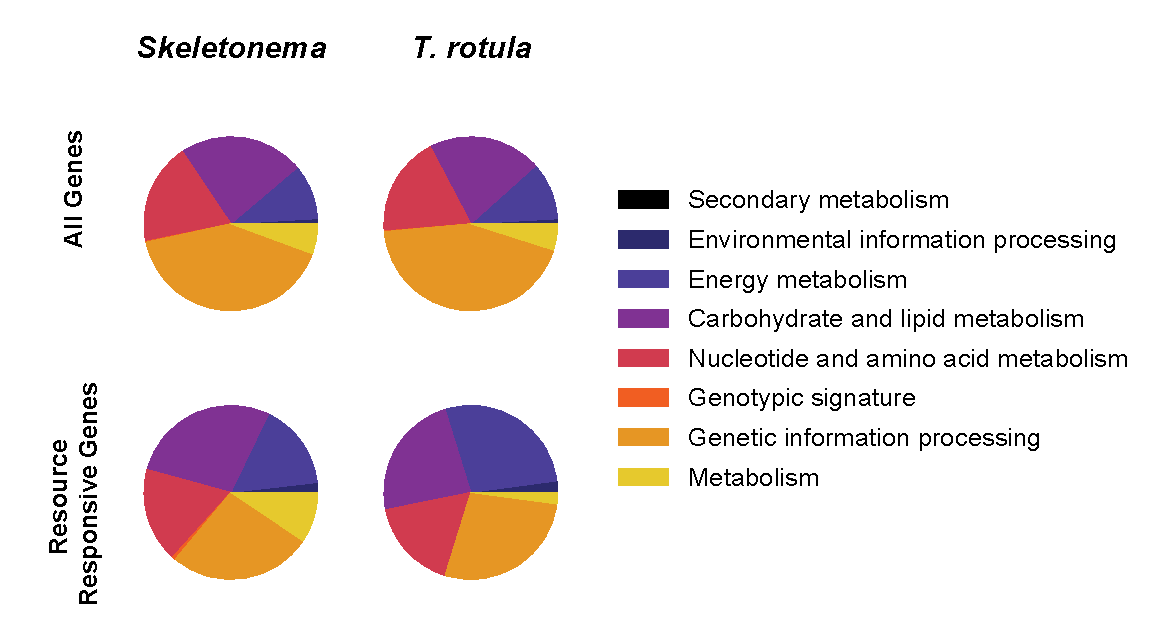
\includegraphics[width=1\textwidth]{Images/C3_SFigure5_RR_All_Genes_Pie.pdf}
    \caption[Functional compoosition of the reference transcriptome and resource-responsive gene sets]{Functional composition of the reference transcriptome and resource-responsive (RR) gene subset for \textit{T. rotula} and \textit{Skeletonema} spp. (A) RR gene sets were identified through cross comparison of like-nutrient incubations (i.e. +N vs. -N and +P vs. -P), using ASC (fold change = 2, post-$p > 0.95$). The relative functional categorization of the reference transcriptomes and RR gene set for \textit{T. rotula} and \textit{Skeletonema} spp. based on KEGG ontology as assigned by KAAS is depicted at the module-level.}
  \label{fig:a3f5}
\end{figure}

%Supplemental Figure 6: Expression of nitrate reductase

\begin{figure}[p!]
  \centering
    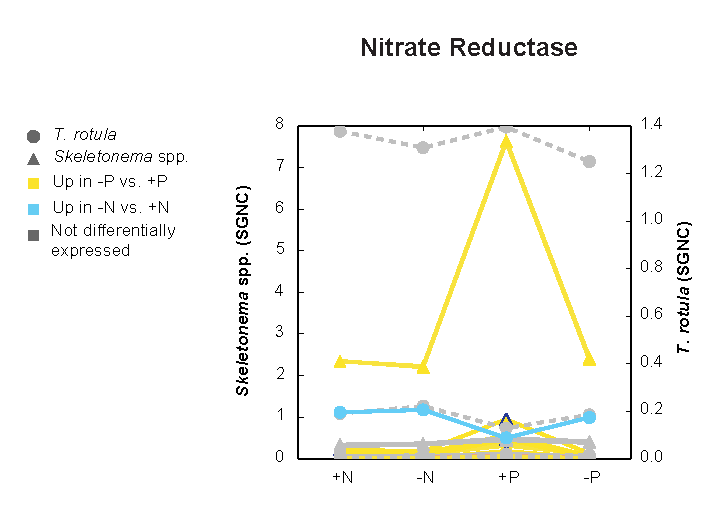
\includegraphics[width=1\textwidth]{Images/C3_SFigure6_SGNC_NitrateReductase.pdf}
    \caption[Relative expression of nitrate reducatses across incubation experiments]{The relative expression in stable gene normalized counts ($SGNC$) of the assimilatory nitrate reductase gene cluster across the incubation experiment treatments. Significance of regulation between the treatments is denoted by the color of the line; organisms are denoted by the shapes of the marker.}
  \label{fig:a3f6}
\end{figure}

%Supplemental Figure 7: Cluster Analysis


\begin{figure}[p!]
  \centering
    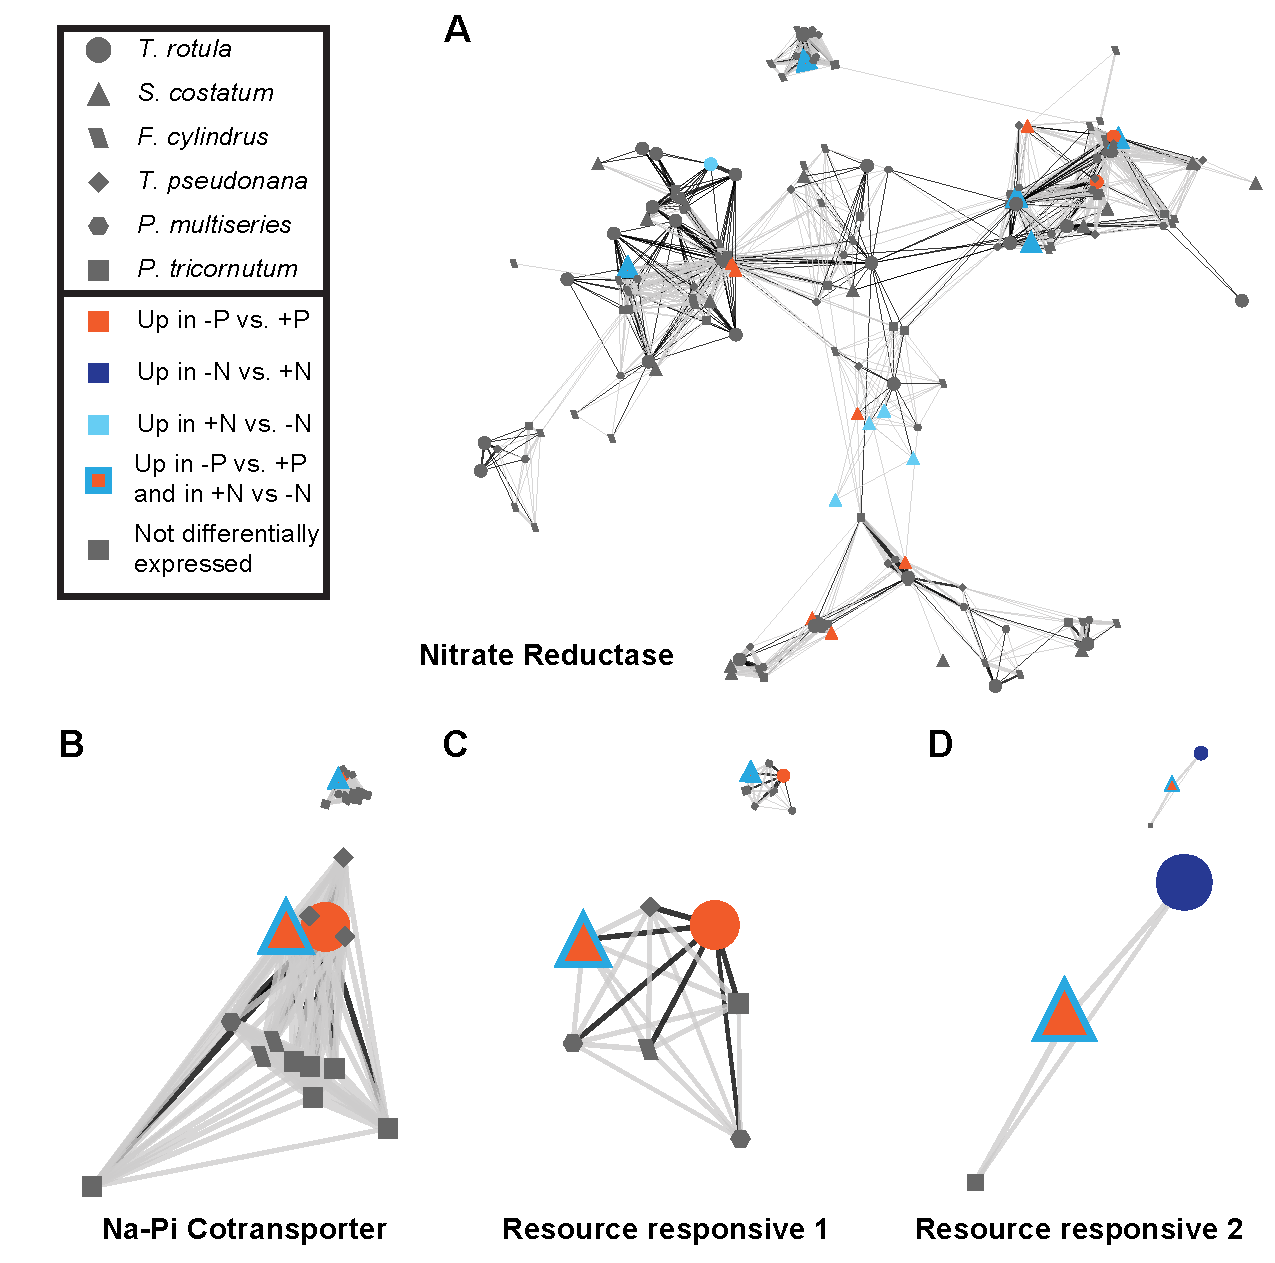
\includegraphics[width=1\textwidth]{Images/C3_SFigure7_ClusterAnalysis_v5.pdf}
    \caption[Gene cluster analysis of nutrient-responsive genes]{Gene cluster known nutrient-responsive genes in \textit{T. pseudonana}: (A) assimilatory nitrate reductase and (B) sodium-phosphate cotransporter and novel resource-responsive (RR) gene families: (C) RR1 and (D) RR2. Transcripts from the transcriptomes of \textit{T. rotula} and \textit{Skeletonema} spp. were clustered based upon relative homology with available diatom genomes: \textit{F. cylindrus}, \textit{P. tricornitum}, \textit{P. multiseries}, and \textit{T. pseudonana}. Symbols indicate different species, while color indicates regulation in the field incubation experiments. Two nodes within a gene cluster are connected by an edge if they share a homologous protein (reciprocal BLAST hit with a minimum of 1e-5 score and minimum 20\% identity). Gene clusters are visualized using an edge-weighted spring-embedded model based on e-value, meaning that genes that are closer together are more similar. The width of the line correlates to the magnitude of the e-value, with lower e-values represented by thicker lines and higher e-values represented by thinner lines.}
  \label{fig:a3f7}
\end{figure}

%Supplemental Figure 8: Conceptual schematic of STD niche space

\begin{figure}[p!]
  \centering
    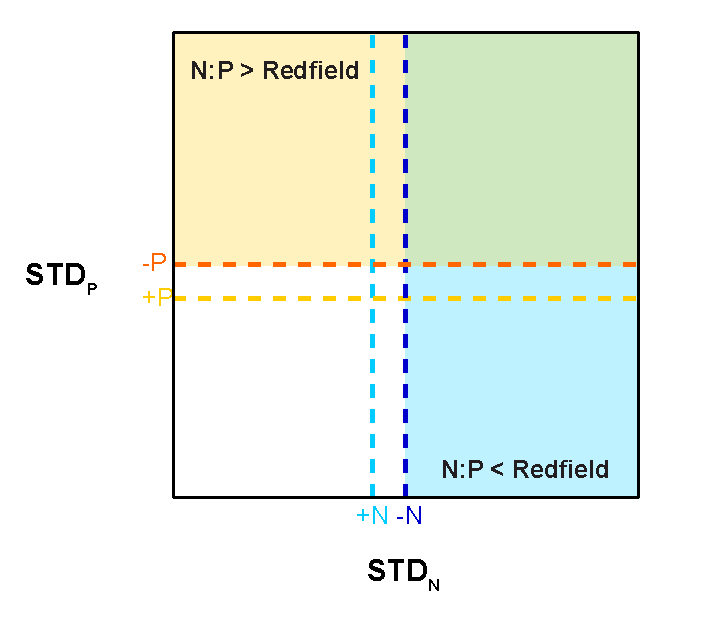
\includegraphics[width=1\textwidth]{Images/C3_SFigure8_Schematic_Quadrants.pdf}
    \caption[Conceptual schemiatic of $STD_N$ plotted against $STD_P$]{A conceptual schematic of $STD_N$ plotted against $STD_P$ hypothesized regions of N:P > Redfield physiology and N:P < Redfield physiology highlighted.}
  \label{fig:a3f8}
\end{figure}


%Supplemental Figure 9: NISP Dn genes
\begin{landscape}
   \centering
   \null         %%<---- this is needed
   \vfill        %%<-----here

	\begin{figure}
  	\centering
    	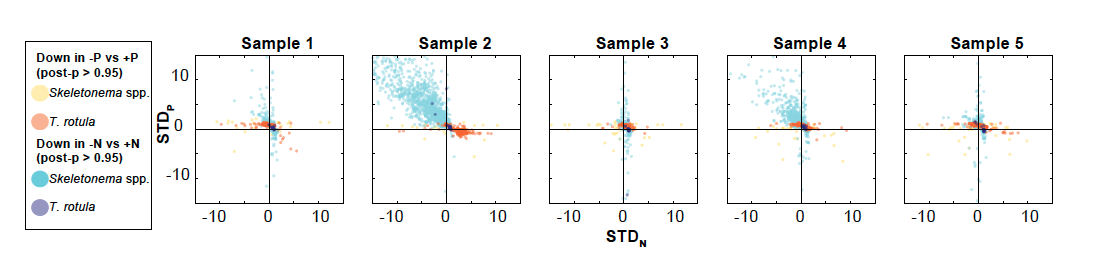
\includegraphics[width=1.3\textwidth]{Images/C3_SFigure9_NISP_DNGenes.png}
    	\caption[Evolution of niche space indexing over for significantly down-regualted genes]{Evolution of niche space indexing over time in Narragansett Bay for \textit{T. rotula} and \textit{Skeletonema} spp.. The stable gene normalized field signal from genes identified as significantly (2-fold change, post$-p > 0.95$) down-regulated in -P vs +P for Skeletonema spp. (yellow) and \textit{T. rotula} (orange) and in -N vs +N for for \textit{Skeletonema} spp. (cyan) and \textit{T. rotula} (dark blue) was proportionalized relative to the expression for those genes in nutrient incubations, yielding the $STD_N$ and $STD_P$. These data are plotted for Sample 1 through Sample 5.}
  	\label{fig:a3f9}
	\end{figure}
    \vfill        %%<----- and here
\end{landscape}

%Supplemental Figure 10: Percentage of RR genes by quadrant

\begin{figure}[h!]
  \centering
    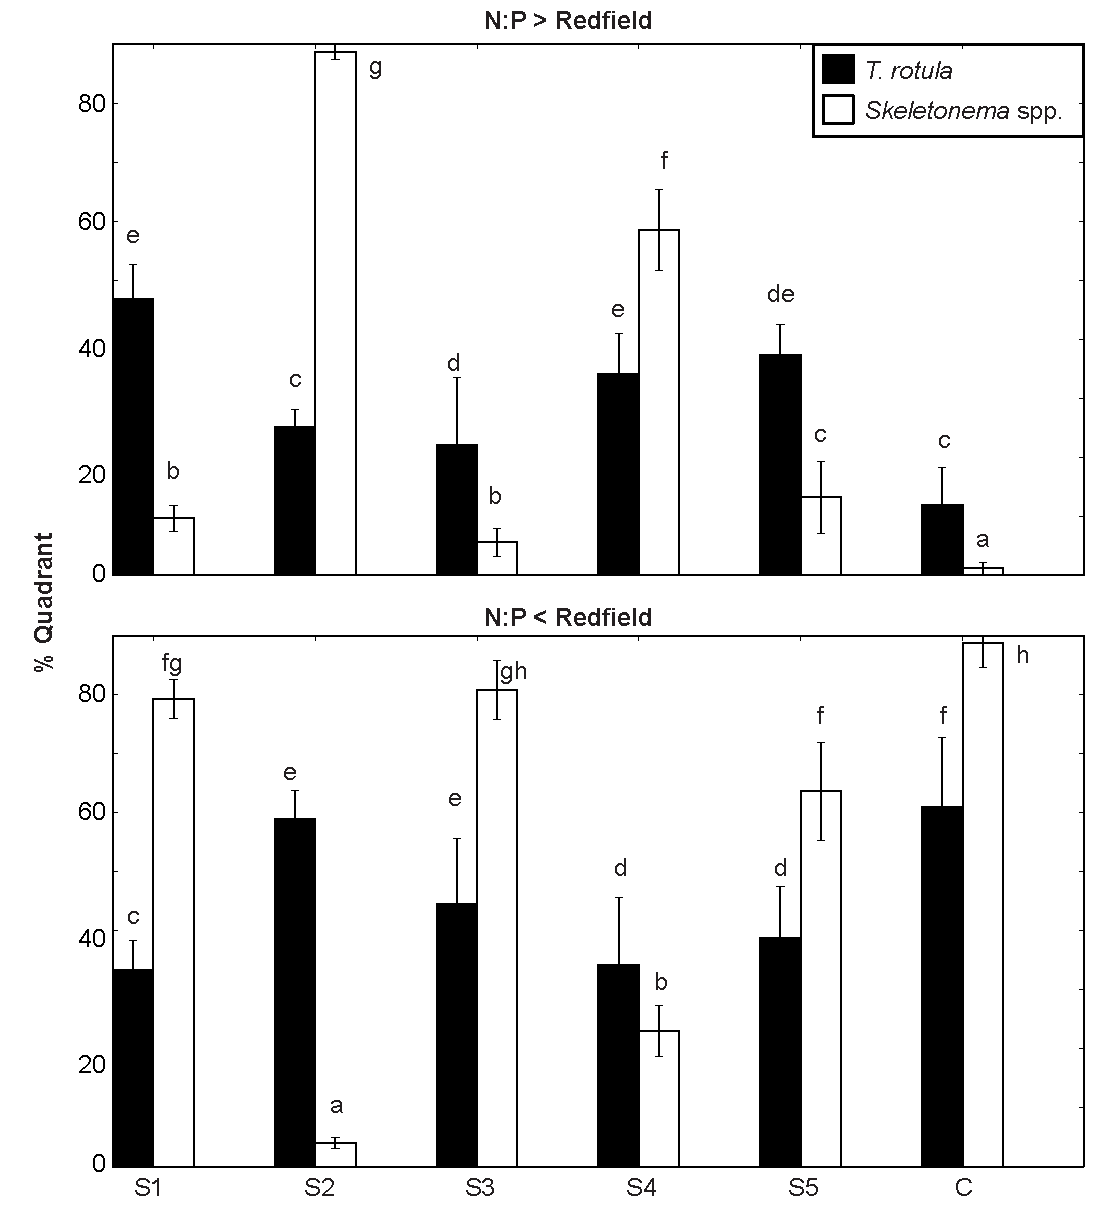
\includegraphics[width=1\textwidth]{Images/C3_SFigure10_BarGraph_Quadrant_2575_stats.pdf}
    \caption[The percentage of identified nutrient responsive genes falling into the N:P > Redfield and N:P < Redfield quadrants with varried cutoffs]{The percentage of identified nutrient responsive genes falling into the N:P > Redfield and N:P < Redfield quadrants for \textit{T. rotula} and \textit{Skeletonema} spp.. The total number of genes falling into the N:P > Redfield quadrant ($STD_P > C$; $STD_N < C$, for $0.25 < C < 0.75$) and the N:P < Redfield quadrant ($STD_P$ < C; $STD_N > C$, for $0.25 < C < 0.75$). The value of C was varied over 10 different values and the average percentages of genes falling into each of the quadrants is depicted above based on the size of the circle at the median $STD_N$ and $STD_P$ for the genes in the quadrant. Similarity of data between species by quadrant was assessed using an analysis of variance (ANOVA) with a generalized linear model. The results from a post hoc Tukey test show the divergence of species across time ($p < 0.05$).}
  \label{fig:a3f10}
\end{figure}

%Supplemental Figure 11: Quadrant localization with varying stable reference genes

\begin{figure}[p!]
  \centering
    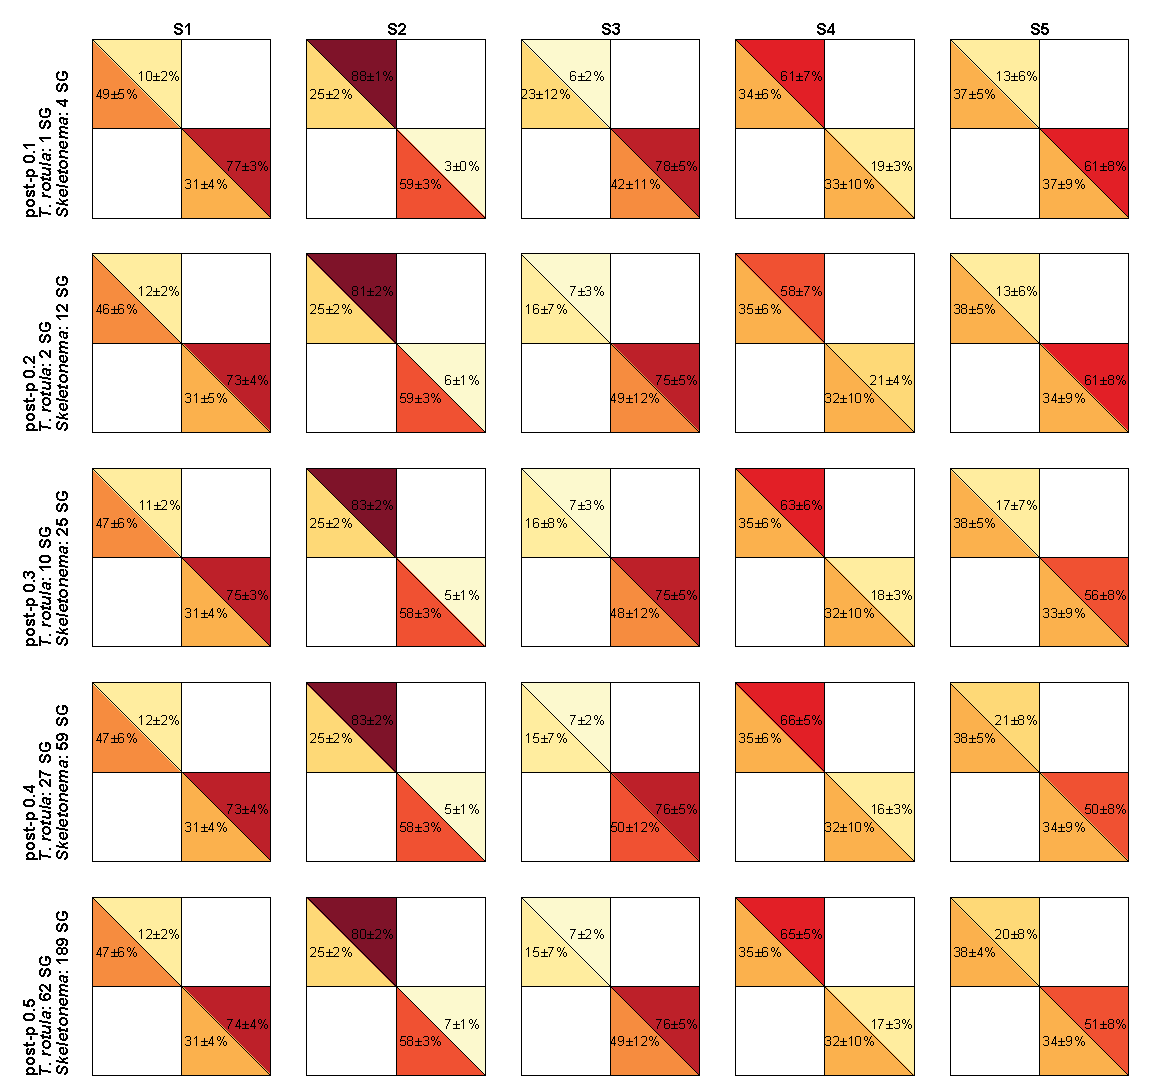
\includegraphics[width=1\textwidth]{Images/C3_SFigure11_Quadrant.pdf}
    \caption[The impact of stable gene selction of quadrant localization]{The impact of stable gene selection on the quadrant localization of the resource responsive gene sets. The posterior probability cutoff used in the selection of stable genes was varied from 0.1 to 0.5 for a fold change of 1.25. The percentage of identified nutrient responsive genes falling into the N:P > Redfield and N:P < Redfield quadrants for \textit{T. rotula} and \textit{Skeletonema} spp. across the five sample points and five posterior probability values is depicted.}
  \label{fig:a3f11}
\end{figure}



\subsection{Supplemental Tables}

%Supplemental Table 1: library stats

\begin{table}[h!]
\centering
\caption[The total number of paired end reads after quality control and trimming and the percentage of reads mapping]{The total number of paired end reads after quality control and trimming and the percentage of reads mapping to the \textit{T. pseudonana} genome, \textit{T. rotula} transcriptome, and \textit{S. costatum} transcriptome.}
\label{tab:a3t1}

\newcolumntype{C}[1]{>{\centering\let\newline\\\arraybackslash\hspace{.5pt}}m{#1}}

\begin{tabular}{|C{2cm}|C{2.5cm}|C{2.5cm}|C{2.5cm}|C{2.5cm}|}
\hline
\multirow{2}{*}{Sample} & \multirow{2}{*}{\parbox{2.5cm}{Total library size (paired end reads)}} & \multicolumn{3}{c|}{Mapped representation in library} \\ \cline{3-5} 
                        &                                                              & \textit{T. pseudonana}      & \textit{T. rotula}      & \textit{S. costatum}     \\ \hline
S1                      & 89455034                                                     & 2.98\%             & 17.50\%        & 33.50\%         \\ \hline
S2                      & 64888267                                                     & 0.41\%             & 11.70\%        & 54.90\%         \\ \hline
S3                      & 103250243                                                    & 0.39\%             & 7.30\%         & 9.00\%          \\ \hline
S4                      & 45370867                                                     & 0.68\%             & 8.80\%         & 8.30\%          \\ \hline
S5                      & 55061692                                                     & 0.88\%             & 10.40\%        & 11.20\%         \\ \hline
Ambient Control         & 51508197                                                     & 0.27\%             & 13.40\%        & 8.00\%          \\ \hline
+N                      & 58626239                                                     & 0.43\%             & 6.10\%         & 5.30\%          \\ \hline
-N                      & 44561851                                                     & 0.41\%             & 8.70\%         & 8.30\%          \\ \hline
+P                      & 51130364                                                     & 0.29\%             & 8.50\%         & 8.00\%          \\ \hline
-P                      & 58834022                                                     & 0.40\%             & 6.60\%         & 6.50\%          \\ \hline
\end{tabular}
\end{table}

%Supplememntal Table 2: nutrient concentrations used in incubations

\begin{table}[h!]
\centering
\caption[Nutrient concentrations used in nutrient amendment incubations. ]{Nutrient concentrations used in nutrient amendment incubations.}
\label{tab:a3t2}
\begin{tabular}{|c|c|c|c|c|c|}
\hline
                                    & \multicolumn{5}{c|}{\textbf{Treatment}}                                                                                              \\ \cline{2-6} 
\multirow{-2}{*}{\textbf{Nutrient}} & Ambient Control          & + P                      & + N                      & - P                      & - N                      \\ \hline
Nitrate                             & \cellcolor[HTML]{C0C0C0} & \cellcolor[HTML]{C0C0C0} & 10 $\mu M$                    & 10 $\mu M$                    & \cellcolor[HTML]{C0C0C0} \\ \hline
Phosphate                           & \cellcolor[HTML]{C0C0C0} & 3 $\mu M$                     & \cellcolor[HTML]{C0C0C0} & \cellcolor[HTML]{C0C0C0} & 3 $\mu M$                     \\ \hline
Silica                             & \cellcolor[HTML]{C0C0C0} & \cellcolor[HTML]{C0C0C0} & \cellcolor[HTML]{C0C0C0} & 68 $\mu M$                    & 68 $\mu M$                    \\ \hline
Iron                                & \cellcolor[HTML]{C0C0C0} & \cellcolor[HTML]{C0C0C0} & \cellcolor[HTML]{C0C0C0} & 4.6 $\mu M$                   & 4.6 $\mu M$                   \\ \hline
Vitamins                            & \cellcolor[HTML]{C0C0C0} & \cellcolor[HTML]{C0C0C0} & \cellcolor[HTML]{C0C0C0} & f/5                      & f/5                      \\ \hline
\end{tabular}
\end{table}


%Supplememntal Table 3: nutrient concentrations used in incubations

\begin{table}[h!]
\centering
\caption[Mapping statistics for \textit{T. rotula} and \textit{S. costatum} transcriptomes]{Total number of contigs in the \textit{T. rotula} and \textit{S. costatum} transcriptomes and the number of genes in each of the differentially regulated and stable groupings.}
\label{tab:a3t3}
\begin{tabular}{|l|l|l|}
\hline
                                                                       & \textit{\textbf{T. rotula}} & \textit{\textbf{S. costatum}} \\ \hline
Number of contigs in transcriptome                                     & 22362                       & 27665                         \\ \hline
Pass 2 TPM cutoff                                                      & 4318                        & 20921                         \\ \hline
Up in -P vs +P                                                         & 249                         & 4754                          \\ \hline
Down in -P vs +P                                                       & 335                         & 52                            \\ \hline
Up in -N vs +N                                                         & 196                         & 9                             \\ \hline
Down in -N vs +N                                                       & 49                          & 1631                          \\ \hline
All differentially regulated (2 fold change, post-$p > 0.95$) & 775                         & 5136                          \\ \hline
Stable genes (1.25 fold change, post-$p < 0.1$)                  & 1                           & 4                             \\ \hline
\end{tabular}
\end{table}

\clearpage

\subsection{Supplemental Data}

\newlist{DS3}{enumerate}{1}
\setlist[DS3]{label=Data Sheet 3-\arabic*}

    \begin{DS3}
    
    \item \label{DS31}: Annotations based on KEGG Ontology for \textit{Skeletonema} spp. and \textit{T. rotula} transcriptomes. \href{http://www.pnas.org/content/suppl/2015/04/09/1421993112.DCSupplemental/pnas.1421993112.sd01.xlsx}{Data Sheet 3-1} can be downloaded from the online version of the manuscript of \citet{Alexander2015} through \href{http://www.pnas.org/content/112/17/E2182.full}{\textit{Proceedings of the National Academy of Sciences}}. 
    \item \label{DS32}: Relative expression in tags per million (TPM) for genes identified as differentially or stably expressed in nutrient incubations. \href{http://www.pnas.org/content/suppl/2015/04/09/1421993112.DCSupplemental/pnas.1421993112.sd02.xlsx}{Data Sheet 3-2} can be downloaded from the online version of the manuscript of \citet{Alexander2015} through \href{http://www.pnas.org/content/112/17/E2182.full}{\textit{Proceedings of the National Academy of Sciences}}. 
  
    \end{DS3}



%%%%%%%%%%%%%%%%%%%%%%%%%%%

%%%%%%%%%%%%%%%%%%%%%%%%%%%_________________CHAPTERFOUR_________________%%%%%%%%%%%%%%%%%%%%%%%%%%%

%%%%%%%%%%%%%%%%%%%%%%%%%%%


\clearpage

\section{Appendix for Chapter 4}
\subsection{Supplemental Figures}

%Supplemental Figure 1: Chlorophyll values in experiments and in situ samples 
\begin{figure}[h!]
  \centering
    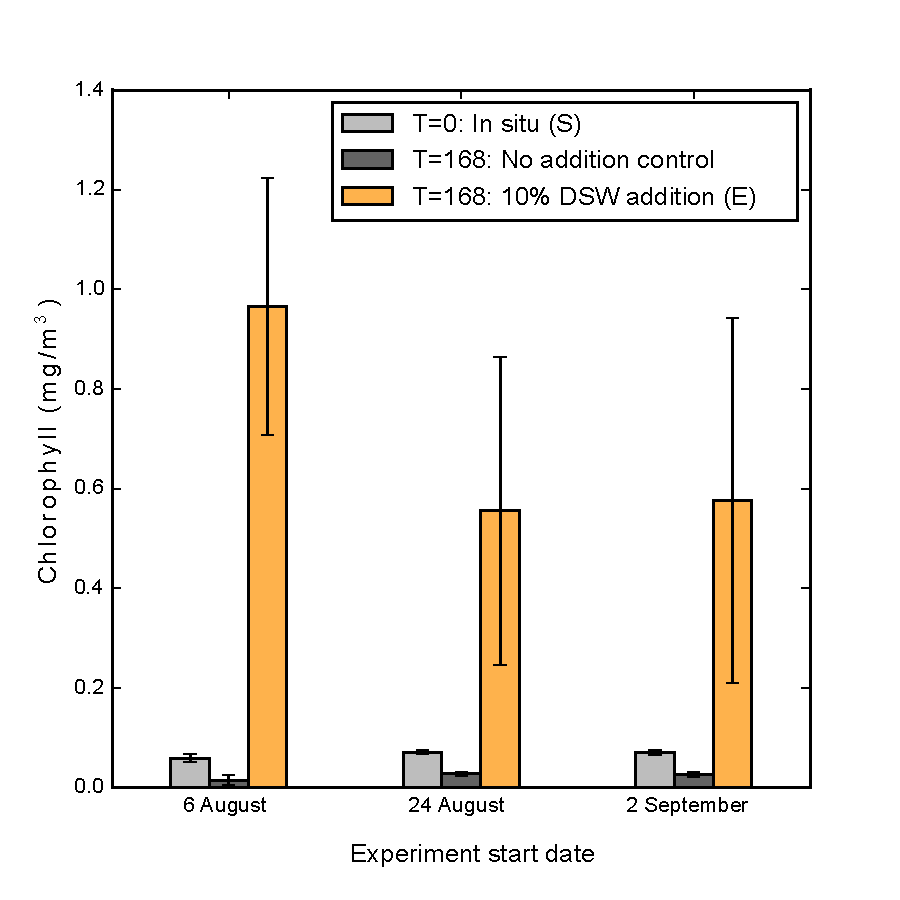
\includegraphics[width=1\textwidth]{Images/C4_FigureS1.pdf}
    \caption[Chlorophyll a of replicated experiments for \emph{in situ} samples, no addition control, and a 10\% deep seawater amendment]{Chlorophyll a of replicated experiments for \emph{in situ} samples (S), a no addition control, and a 10\% deep seawater (DSW) amendment (E). Incubation samples were harvested after 168 hours.}
  \label{fig:a4f1}
\end{figure}


%Supplemental Figure 2: Rank abundance shifts in species composition of diatoms, haptophytes and dinoflagellates

\begin{landscape}
 %  \null         %%<---- this is needed
   \vfill        %%<-----here
\begin{figure}[p!]
  \centering
    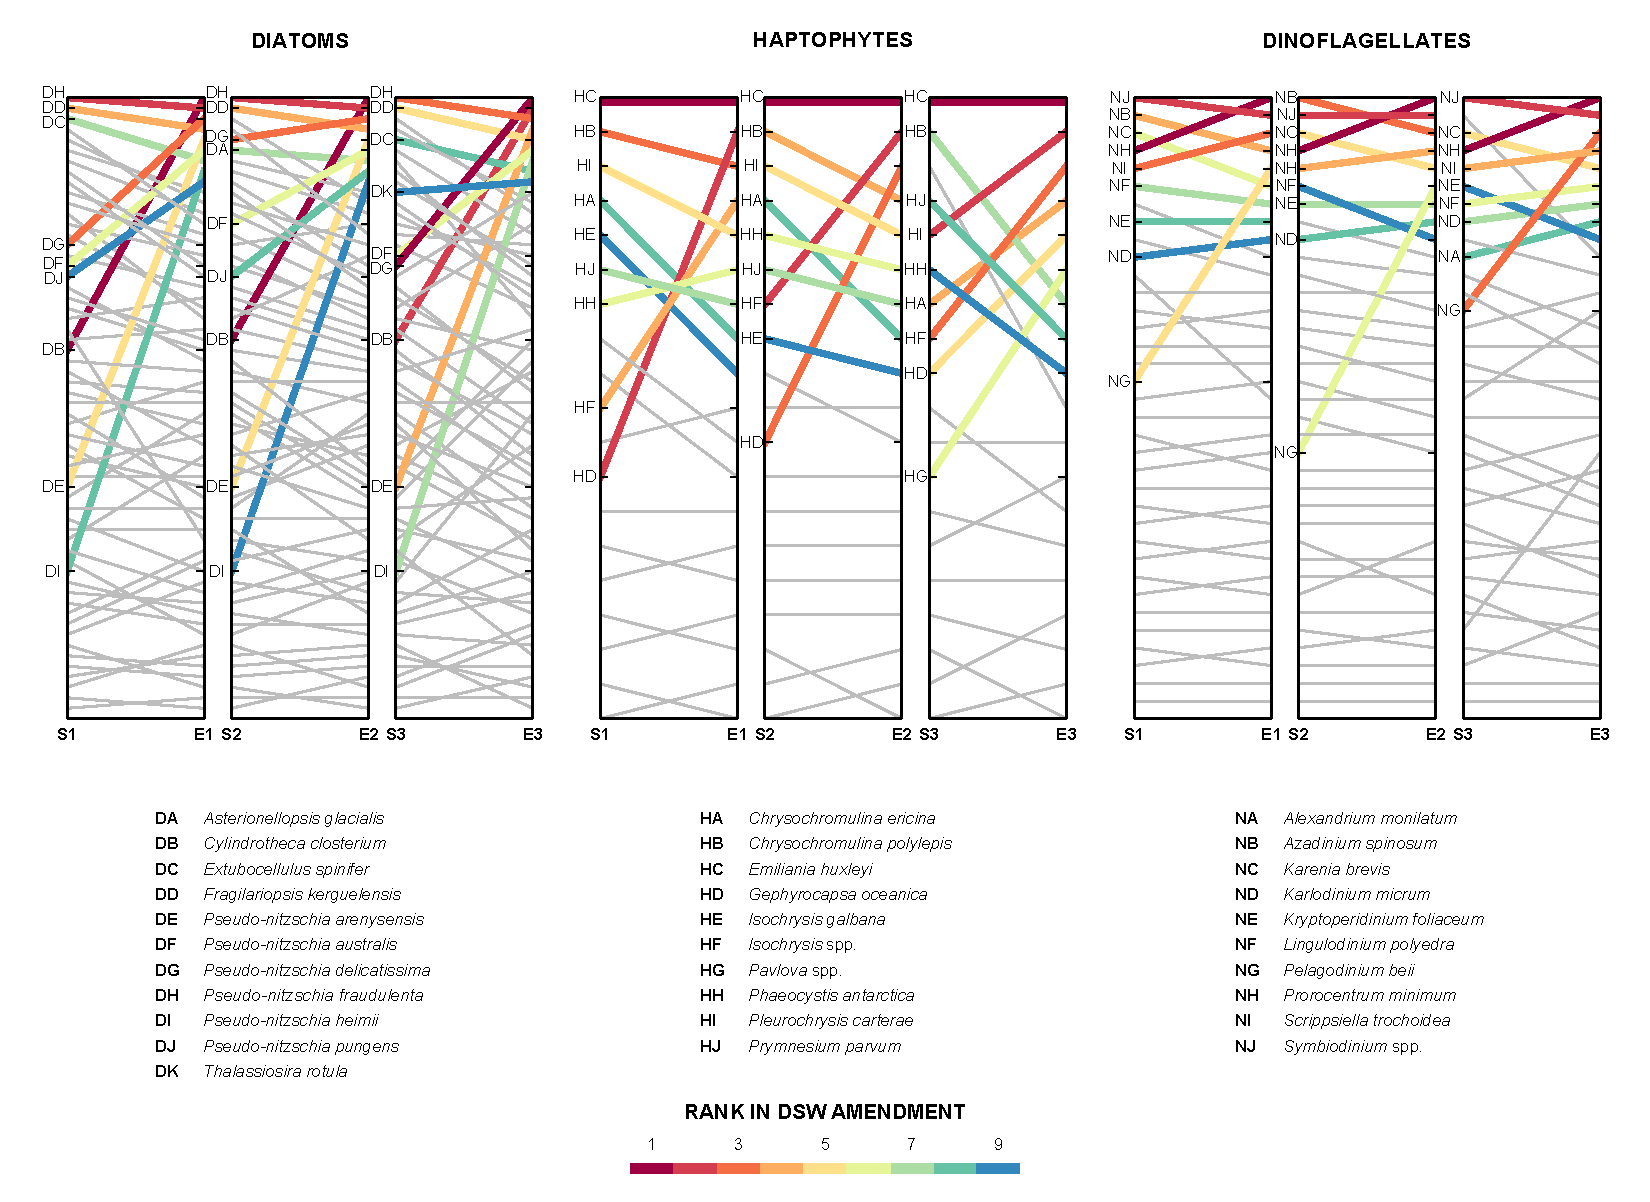
\includegraphics[width=1\textwidth]{Images/C4_FigureS2.pdf}
    \caption[Rank abundance shifts in the species composition of diatoms, haptophytes and dinoflagellates]{Rank abundance shifts in the species composition of diatoms, haptophytes and dinoflagellates for the three experiments. The relative shift in rank abundance for each species is depicted for each incubation experiment (E1-E3) following deep seawater (DSW) addition. The nine most abundant taxa following DSW addition are highlighted for each of the functional groups. Although the species that recruited the reads are denoted here this is highly driven by the composition of the database and does not necessarily indicate the actual species present, but rather the closest species present in the database.}
  \label{fig:a4f2}
\end{figure}
    \vfill        %%<----- and here
\end{landscape}


%Supplemental Figure 3: QMF Comparison across species


\begin{figure}[p!]
  \centering
    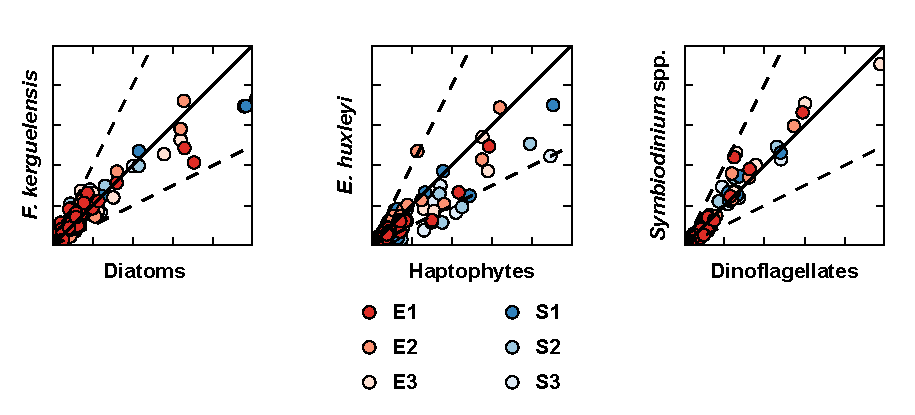
\includegraphics[width=1\textwidth]{Images/C4_FigureS3.pdf}
    \caption[Comparison of the quantitative metabolic fingerprint (QMF) between the whole functional group and representative taxa]{Comparison of the quantitative metabolic fingerprint (QMF) between the whole functional group and representative taxa. The proportion of reads falling into each of the modules depicted in Figure 2 is plotted for S1-S3 and E1-E3, comparing the summed functional group signal and that of a representative taxon. Color of the marker indicates the sample; solid and dashed lines mark the 1:1 and 1:2 lines, respectively.}
  \label{fig:a4f3}
\end{figure}

%Supplemental Figure 4: Distribution histogram

\begin{figure}[p!]
  \centering
    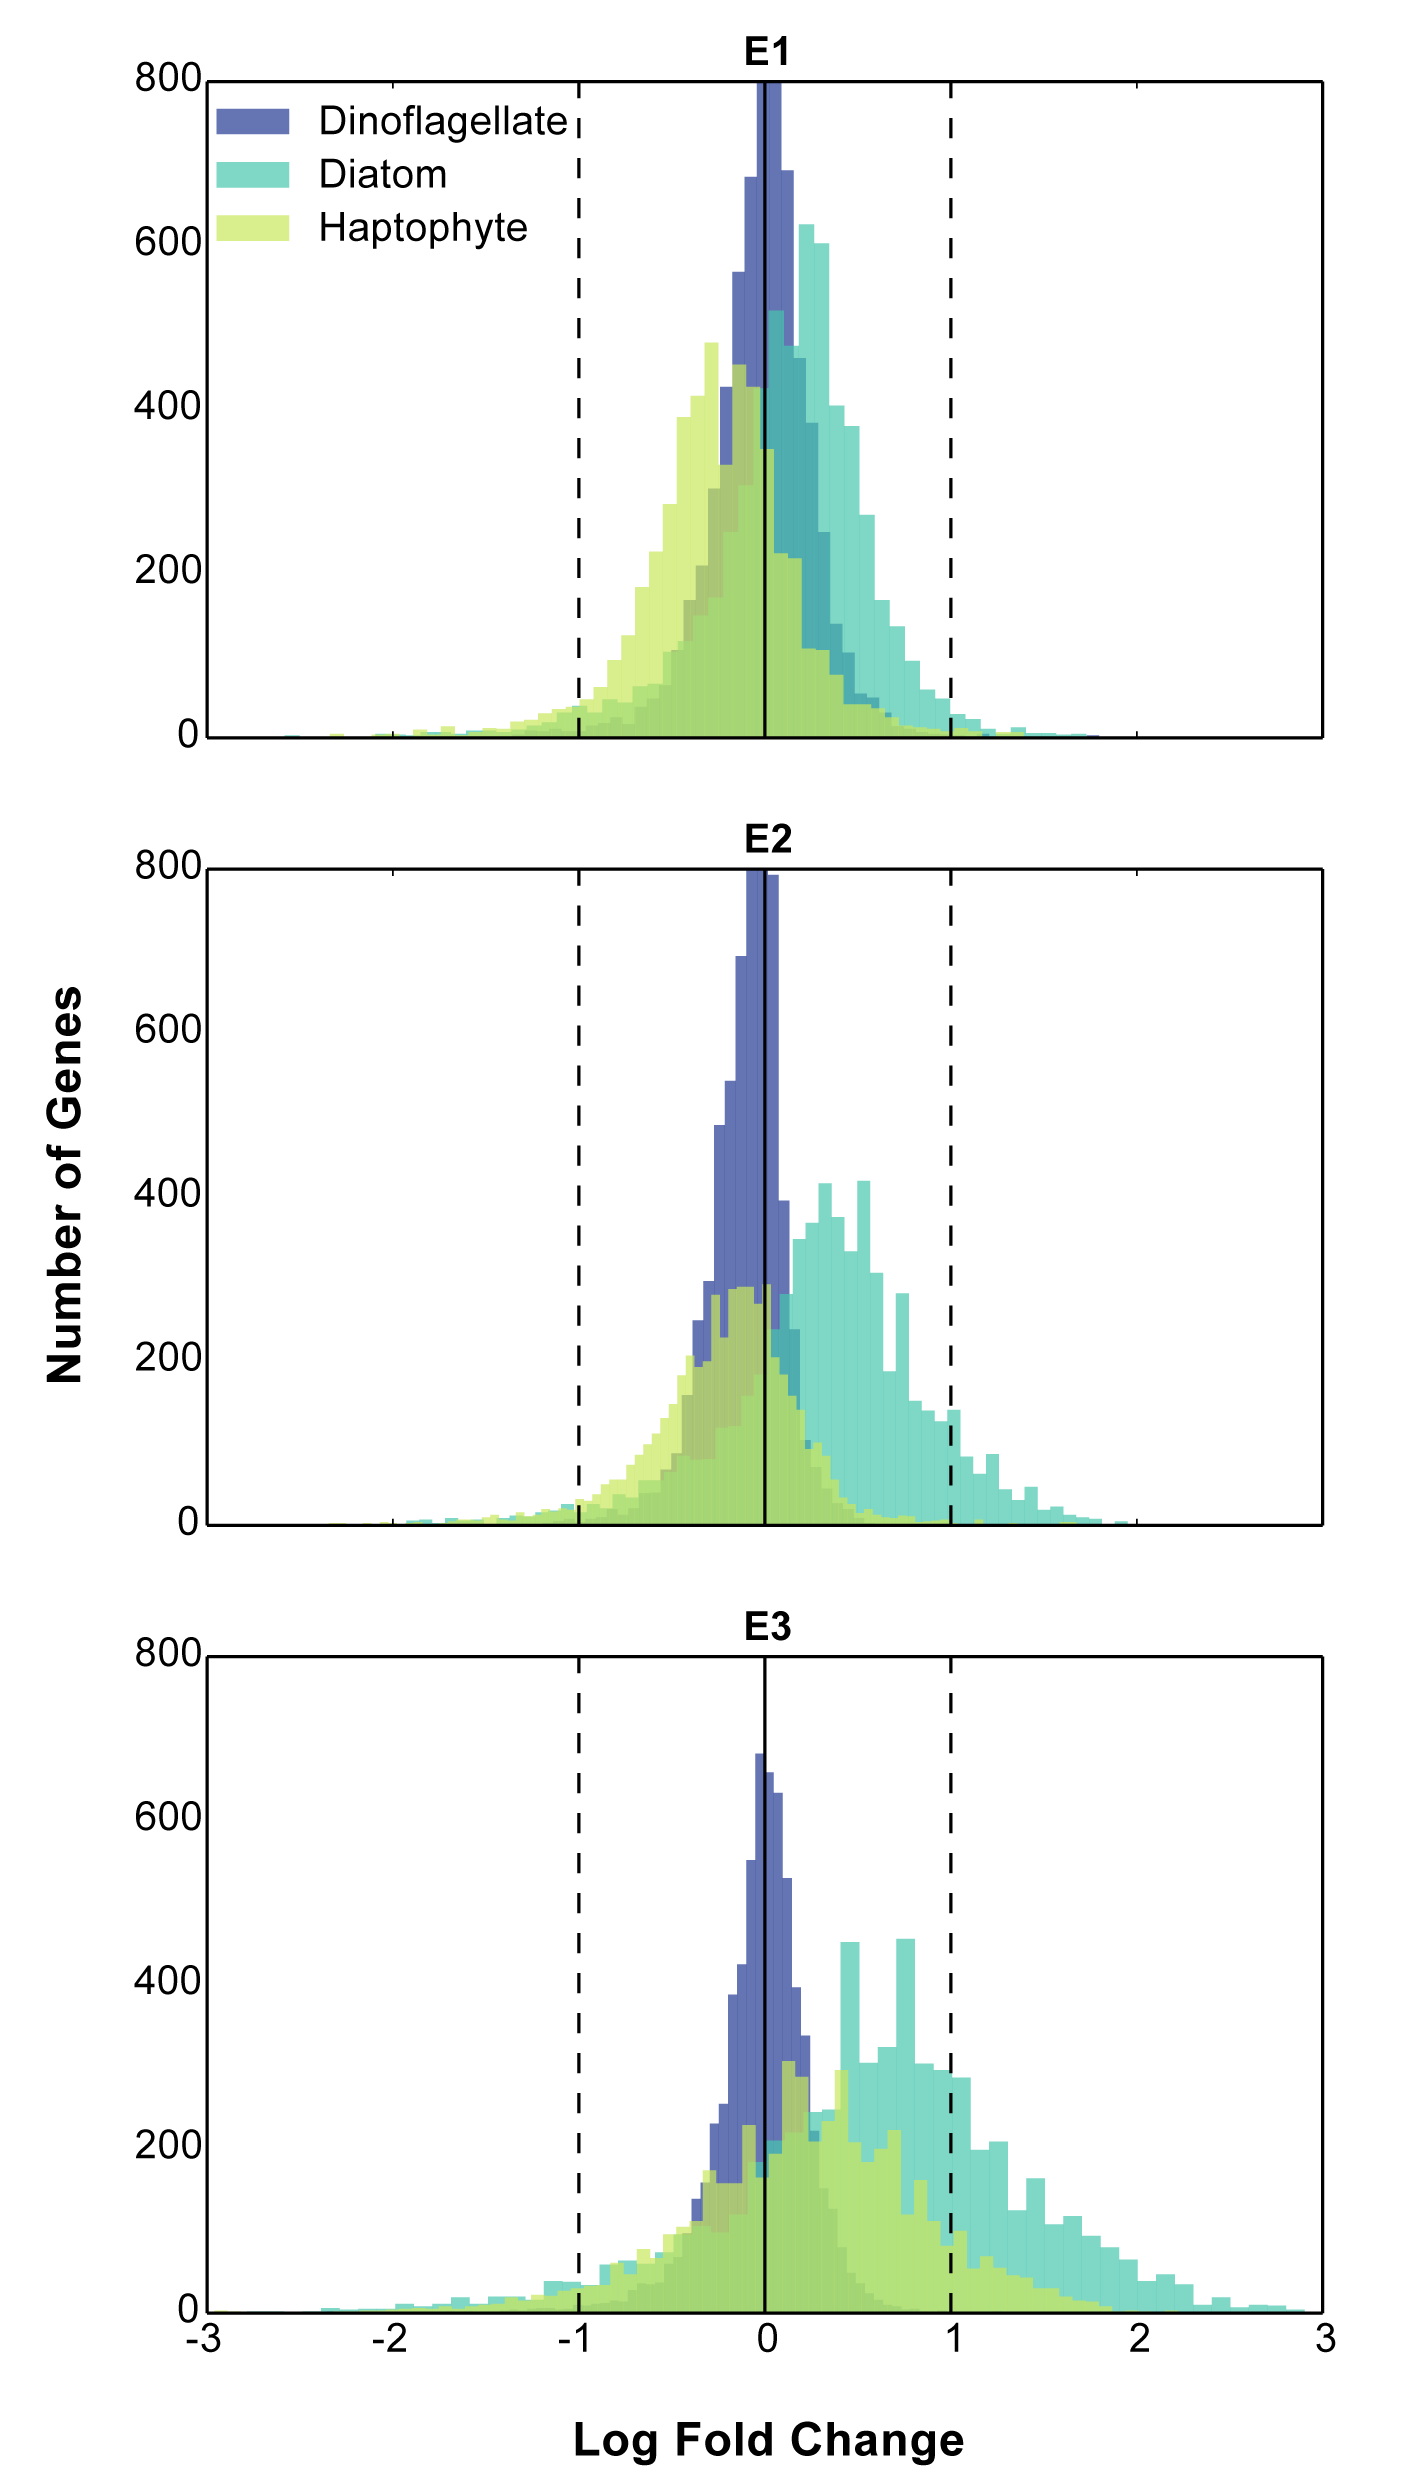
\includegraphics[width=.75\textwidth]{Images/C4_FigureS4.png}
    \caption[Distribution of log fold change following deep seawater (DSW) addition]{Distribution of log fold change following deep seawater (DSW) addition. Histogram of the number of genes falling within each of the log fold change bins for diatoms, haptophytes and dinoflagellates. Solid line indicates no fold change; dashed lines indicate 2 fold-change both up and down.}
  \label{fig:a4f4}
\end{figure}


%Supplemental Figure 5: Weight venn diagrams for up and down regulated genes

\begin{figure}[p!]
  \centering
    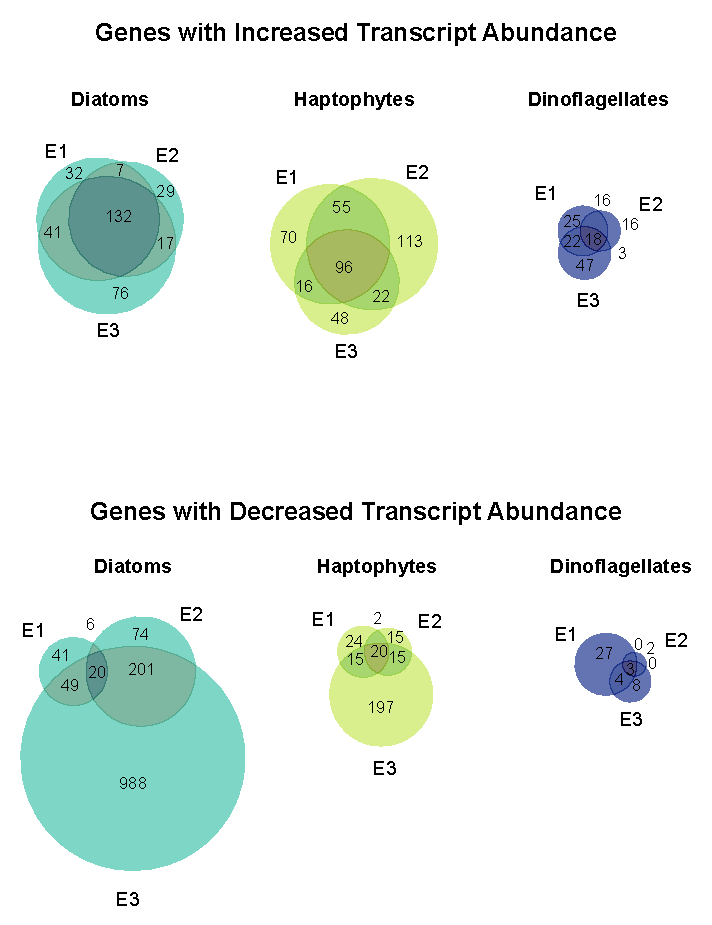
\includegraphics[width=1\textwidth]{Images/C4_FigureS5.pdf}
    \caption[Weighted Venn diagrams of genes with significantly different abundances following deep seawater (DSW) addition by functional group]{Weighted Venn diagrams of genes with significantly different abundances following deep seawater (DSW) addition by functional group. The uniqueness of KEGG orthologs with increased or decreased abundances as determined by ASC (2 fold-change, post-p > 0.95) across experiments was assessed for diatoms, haptophytes, and dinoflagellates.}
  \label{fig:a4f5}
\end{figure}


%Supplemental Figure 6: MANTA Plots

\begin{figure}[p!]
  \centering
    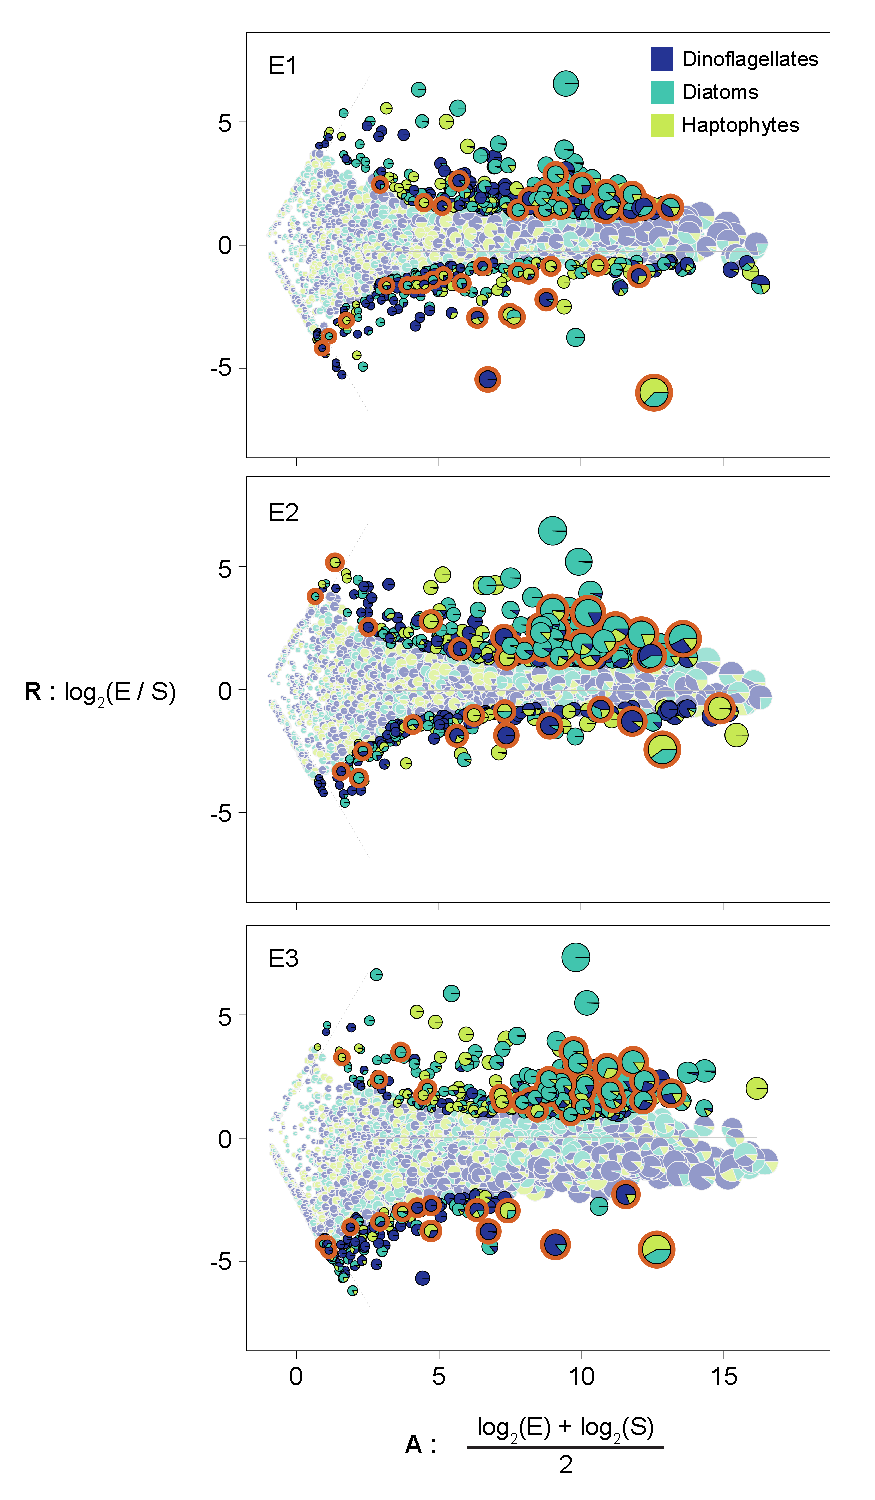
\includegraphics[width=.7\textwidth]{Images/C4_FigureS6.pdf}
    \caption[Microbial Assemblage Normalized Transcript Analysis (MANTA) ratio-averaged plots for global shifts in expression of KEGG orthologs]{Microbial Assemblage Normalized Transcript Analysis (MANTA) ratio-averaged plots for global shifts in expression of KEGG orthologs. Fold change ratio (R) and average read count (A) are plotted for read counts in the \emph{in situ} (S) and deep seawater (DSW) amendment (E) samples across the three sample pairs (S1:E1, S2:E2, S3:E3). The trimmed mean of fold-change values is noted as a gray solid line; orthologs unique to one library are separated by gray dashed lines. Pies indicate the taxonomic distribution of orthologous reads across the three functional groups. KEGG orthologs that were significantly differentially expressed (DE) (adjusted $P > 0.05$) are outlined in black and those not significantly DE are outlined in gray. DE KEGG orthologs that fall in the Energy Metabolism KEGG module are outlined in orange.}
  \label{fig:a4f6}
\end{figure}

%Supplemental Figure 7: QMF across incubation experiments

\begin{figure}[p!]
  \centering
    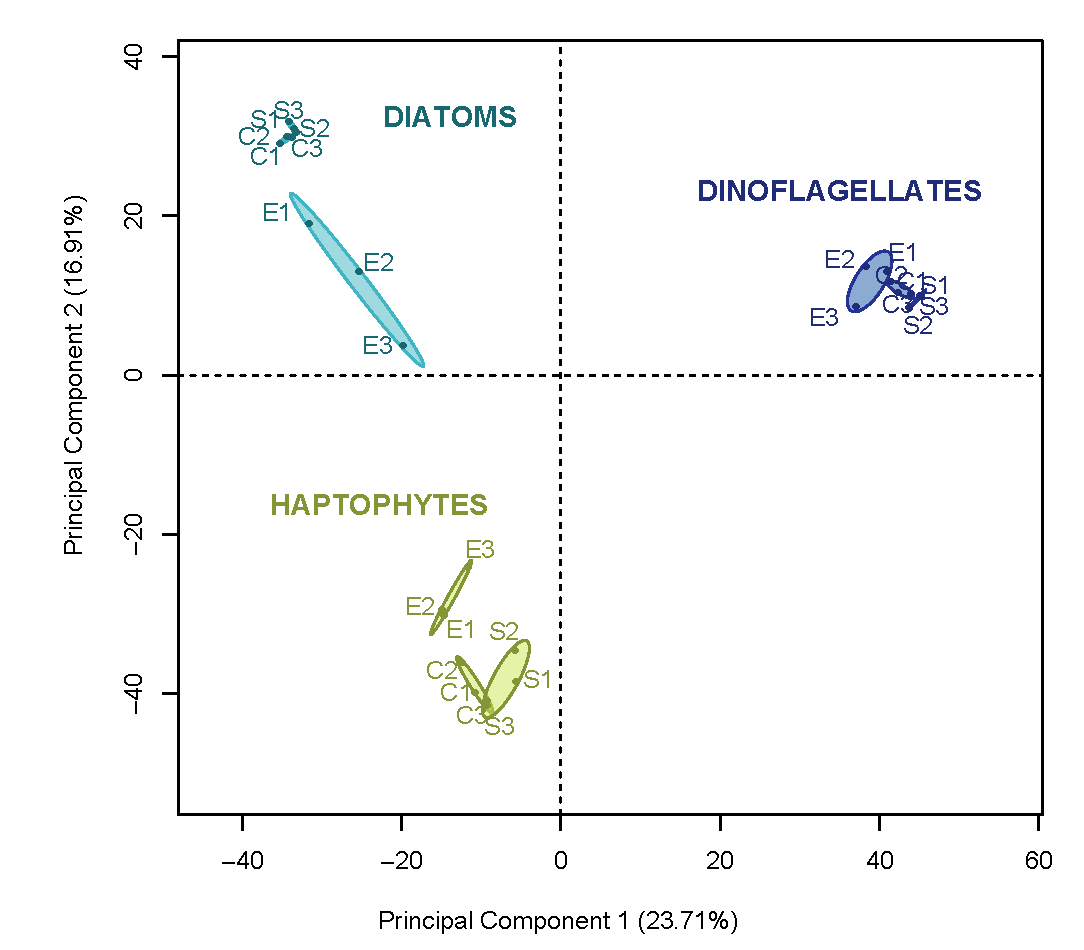
\includegraphics[width=1\textwidth]{Images/C4_FigureS7.pdf}
    \caption[Principal component analysis of the quantitative metabolic fingerprint (QMF) signals across \emph{in situ}, no addition control, and deep seawater amended samples]{Principal component analysis of the quantitative metabolic fingerprint (QMF) signals across \emph{in situ}, no addition control, and deep seawater (DSW) amended samples. Principal component analysis of the QMF signals for each of the functional groups across \emph{in situ} (S1-S3), control no addition (C1-C3) and DSW amendment (E1-E3); 95\% confidence ellipses are indicated for each of the sample types by functional group.}
  \label{fig:a4f7}
\end{figure}

\clearpage

\subsection{Supplemental Tables}

% Supplemental table with nutrient concentrations post treatment run for E and C
\begin{table}[h!]
\centering
\caption[Macronutrient concentrations in deep seawater ammendment and the incubation experiments after 168 hours]{Macronutrient concentrations in control no addition (C), DSW-amended incubations (E), and 700 m water used in DSW amendment incubations}
\label{tab:a4t1}
\newcolumntype{C}[1]{>{\centering\let\newline\\\arraybackslash\hspace{.5pt}}m{#1}}
\begin{tabular}{ccccc}

    
\hline
\multicolumn{1}{|c|}{\multirow{2}{*}{\textbf{Treatment}}} & \multicolumn{1}{c|}{\multirow{2}{*}{\textbf{\begin{tabular}[c]{@{}c@{}}Time post \\ inoculation (hours)\end{tabular}}}} & \multicolumn{1}{c|}{\multirow{2}{*}{\textbf{\begin{tabular}[c]{@{}c@{}}NO2 + NO3 \\ ($\mu M$)\end{tabular}}}} & \multicolumn{1}{c|}{\multirow{2}{*}{\textbf{\begin{tabular}[c]{@{}c@{}}PO4 \\ ($\mu M$)\end{tabular}}}} & \multicolumn{1}{c|}{\multirow{2}{*}{\textbf{\begin{tabular}[c]{@{}c@{}}Si\\ ($\mu M$)\end{tabular}}}} \\

\multicolumn{1}{|c|}{}                                    & \multicolumn{1}{c|}{}                                                        & \multicolumn{1}{c|}{}                                                                                    & \multicolumn{1}{c|}{}                                                                              & \multicolumn{1}{c|}{}                                                                            \\ \hline
\multicolumn{1}{|c|}{\textbf{C} (control no addition) *}  & \multicolumn{1}{c|}{168}                                                     & \multicolumn{1}{c|}{$0.12 \pm 0.03$}                                                                         & \multicolumn{1}{c|}{$0.12 \pm 0.02$}                                                                   & \multicolumn{1}{c|}{$1.91 \pm 0.2$}                                                                  \\ \hline
\multicolumn{1}{|c|}{\textbf{E} (+ 10\% DSW) *}           & \multicolumn{1}{c|}{168}                                                     & \multicolumn{1}{c|}{$1.9 \pm  .93$}                                                                          & \multicolumn{1}{c|}{$0.23 \pm 0.05$}                                                                   & \multicolumn{1}{c|}{$8.46 \pm 3.11$}                                                                 \\ \hline
\multicolumn{1}{|c|}{\textbf{DSW} (700 m water) *}        & \multicolumn{1}{c|}{N/A}                                                     & \multicolumn{1}{c|}{$37.5 \pm 1.68$}                                                                         & \multicolumn{1}{c|}{$3.14 \pm 0.03$}                                                                   & \multicolumn{1}{c|}{$83.4 \pm 9.33$}                                                                 \\ \hline
\multicolumn{5}{l}{\textit{* Nutrient data averaged for E1 and E2, nutrients were not assayed on E3.}}                                                                                                                                                                                                                                                                                                                                                     
\end{tabular}
\end{table}

